% Latex template: mahmoud.s.fahmy@students.kasralainy.edu.eg
% For more details: https://www.sharelatex.com/learn/Beamer

\documentclass[aspectratio=169]{beamer}            % Document class

\usepackage[portuguese]{babel}          % Set language
\usepackage[utf8x]{inputenc}            % Set encoding

\mode<presentation> {                   % Set options
  \usetheme{default}                    % Set theme
  \usecolortheme{default}               % Set colors
  \usefonttheme{default}                % Set font theme
  \setbeamertemplate{caption}[numbered]	% Set caption to be numbered
}

\setbeamertemplate{navigation symbols}{}
\setbeamertemplate{footline}[frame number]
\setbeamercovered{transparent}

\newcommand\Wider[2][3em]{%
\makebox[\linewidth][c]{%
  \begin{minipage}{\dimexpr\textwidth+#1\relax}
  \raggedright#2
  \end{minipage}%
  }%
}

% Uncomment this to have the outline at the beginning of each section highlighted.
%\AtBeginSection[]
%{
%  \begin{frame}{Outline}
%    \tableofcontents[currentsection]
%  \end{frame}
%}

\usepackage{graphicx}                   % For including figures
\usepackage{booktabs}                   % For table rules
\usepackage{hyperref}                   % For cross-referencing
\usepackage{caption}        
\usepackage{siunitx}% Allows more control over captions in figs and tables

\title{Revisão de Atividades da FAC}	% Presentation title
%\author{Author One}					% Presentation author
\institute{LNLS.DAC.FAC}				% Author affiliation
\date{2024-05-10 -- 2024-05-31}			% Today's date	


\begin{document}



\begin{frame}
  \titlepage
  \href{https://github.com/lnls-fac/doc-review-dac-fac}{\beamergotobutton{Link para o repo github desta apresentação: https://github.com/lnls-fac/doc-review-dac-fac}}
  \href{https://www.overleaf.com/read/sbdjxtzfchrm}{\beamergotobutton{Link para o projeto overleaf destas notas}}
\end{frame}

\begin{frame}{Outline}
  \tableofcontents
\end{frame}


% Machine studies in the period
% =============================
% 2024-05-13-SI_ICTs
% 2024-05-13-SI_max_stored_current_estimate
% 2024-05-14-BO_interlock
% 2024-05-14-SI_60hz_ff_orbit
% 2024-05-14-SI_NLK

%====================================================================
\section{Melhorias dos ICTs do LI, TB e TS}

\begin{frame}{Melhorias dos ICTs do LI, TB e TS}

{\footnotesize
\begin{itemize}
    % \setlength\itemsep{1em}
    \item Estudo dia 2024-05-13
    \item Levantamos as curvas cargas nos ICTs do LI vs Tensão de bias no EGun, antes e depois spliting para as eletrônicas Bergoz.
    \item Com o sinal das eletrônicas bergoz ativos, estudar durante turno de usuário.
    \item Medidas de resistência de aterramento e ruídos
\end{itemize}
}
\begin{figure}[ht]
    \begin{minipage}[b]{0.45\linewidth}
        \centering
        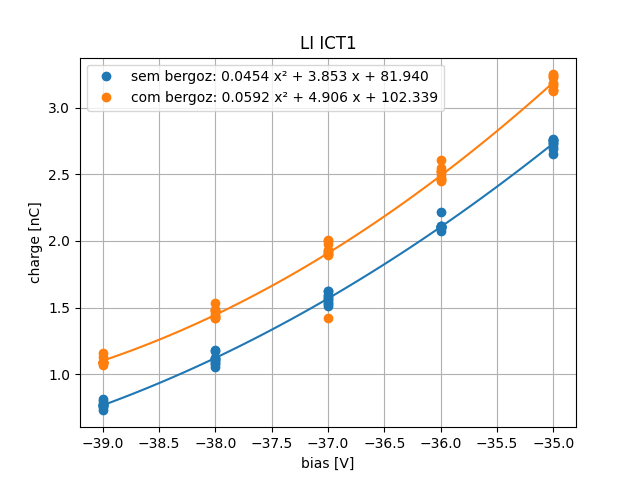
\includegraphics[width=\textwidth]{2024-05-31/figures/li-ict1.png}
        \caption{Calibration of LI ICT1.}
        \label{fig:a}
    \end{minipage}
    \hspace{0.5cm}
    \begin{minipage}[b]{0.45\linewidth}
        \centering
        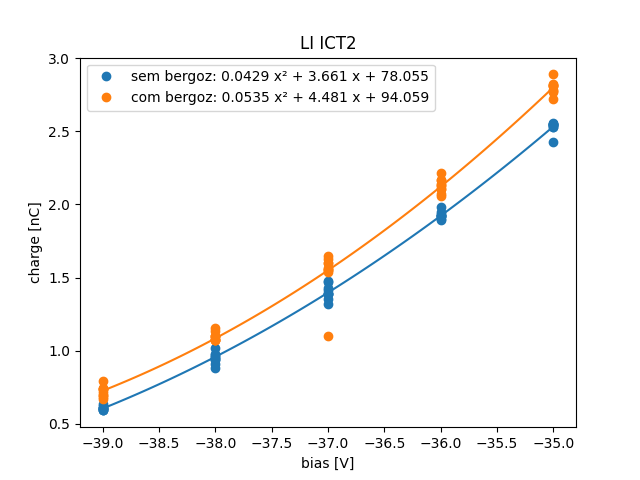
\includegraphics[width=\textwidth]{2024-05-31/figures/li-ict2.png}
        \caption{Calibration of LI ICT2.}
        \label{fig:b}
    \end{minipage}
\end{figure}
\end{frame}

\begin{frame}{Melhorias dos ICTs do LI, TB e TS}
\vspace{0.2cm}
Medidas de resistência de aterramento
\vspace{0.2cm}
{\footnotesize
\begin{itemize}
    \setlength\itemsep{1em}
    \item Entre barras de aterramento no LI, 1 Ohm,
    \item Entre barras e estrutura aceleradora, oscilando em torno de 1.2 Ohm
    \item A barra de aterramento próxima ao BPM 1-02 da TB não há nada conectado a ela e ela também não está aterrada.
    \item As medidas de resistência da câmara do booster em relação ao aterramento variam em torno 1.4 Ohm em trechos distintos 
aumentando até 6 Ohm quando se afasta do trecho de injeção, onde os magnetos pulsados estão conectados ao aterramento.
    \item Próximo ao trecho 04 do anel, tem um cabo que vem da sala de racks e está conectado ao aterramento sem um terminal, parecendo
    precária a conexão.
    \item A resistência entre anel e booster, variam entre 2 e 6 Ohm, diminuido nas proximidades onde o booster etá aterrado.
\end{itemize}
}
\end{frame}

\begin{frame}{Melhorias dos ICTs do LI, TB e TS}
\vspace{0.2cm}
Ruídos
\vspace{0.2cm}
\begin{itemize}
    \setlength\itemsep{1em}
    \item Fizemos diversas medidas do ruído induzido pelo septum, e os ICT's:
    \item Desconectamos o cabo de cada ICt separadamente, com o ímã pulsando e nenhum sinal do pulsador foi observado, conectando
    ou não ma malha externa do cabo coaxial. Mostrando que não é um sinal irradiado.
     \item Deconectamos todos os cabos inclusive os de sincronismo e conexão com a ethernet, e o sinaldo pulsador pode ainda ser observado
\end{itemize}
\end{frame}



%====================================================================
\section{Estimativa de corrente máxima}

\begin{frame}{Estimativa de corrente máxima}

{\footnotesize
\begin{itemize}
    % \setlength\itemsep{1em}
    \item Estudo dia 2024-05-13
\end{itemize}
}
% \begin{figure}[ht]
%     \begin{minipage}[b]{0.45\linewidth}
%         \centering
%         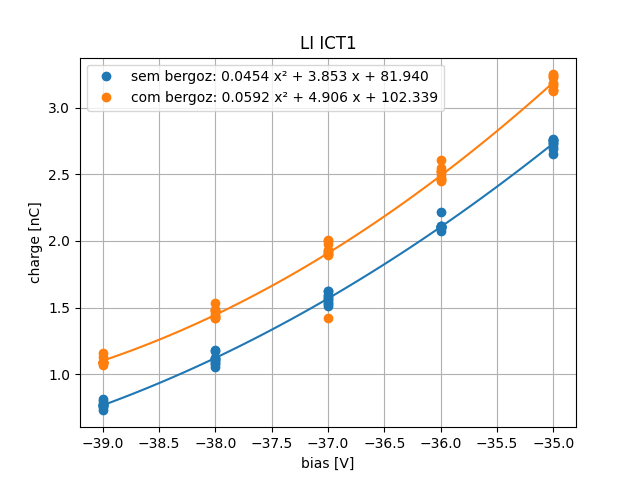
\includegraphics[width=\textwidth]{2024-05-31/figures/li-ict1.png}
%         \caption{Calibration of LI ICT1.}
%         \label{fig:a}
%     \end{minipage}
%     \hspace{0.5cm}
%     \begin{minipage}[b]{0.45\linewidth}
%         \centering
%         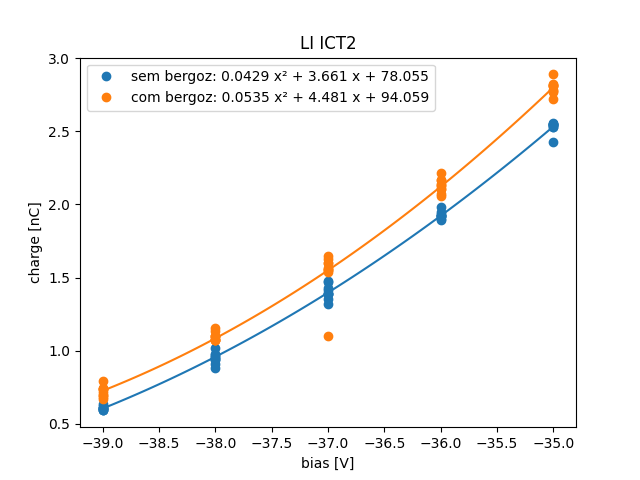
\includegraphics[width=\textwidth]{2024-05-31/figures/li-ict2.png}
%         \caption{Calibration of LI ICT2.}
%         \label{fig:b}
%     \end{minipage}
% \end{figure}
\end{frame}



%====================================================================
\section{FF de órbita para perturbação em 60 Hz}

\begin{frame}{FF de órbita para perturbação em 60 Hz}

\begin{itemize}
    \setlength\itemsep{1em}
    \item Estudos em 2024-05-14
\end{itemize}

\end{frame}



%====================================================================
\section{Migração do shared/screens-iocs}

\begin{frame}{Migração do shared/screens-iocs}

{\footnotesize 
\begin{itemize}
    \setlength\itemsep{1em}
    \item Em 9/04 Eduardo notificou que um volume dos desktops da sala de controle, que pertencem ao GlusterFS, já estava com 81\% de ocupação;
    \item Iniciamos a atividade de migrar a pasta /shared para o Ibirá, acessando da sala de controle via partição montada NFS
    \item De lá pra cá, falhas no NFS que afetaram o acesso tanto durante nossos testes quanto pelas linhas de luz!
    \item Em 09/05 durante testes de cópia do conteúdo do /shared e configuração de permissões, junto à equipe do eduardo, observamos correlação entre nossos testes e problemas de acesso pelas linhas.
    \item Interrompemos a atividade até que o grupo do Eduardo pudesse repensar como configurar permissões para a particularidade de usuário fora de domínio do sirius.
\end{itemize}
}

\end{frame}



%====================================================================
\section{Archiver}

\begin{frame}{Archiver}

{\footnotesize 
\begin{itemize}
    \setlength\itemsep{1em}
    \item Storage tem 64 Tb, 6 Tb disponíveis hoje ($\approx$ 3 meses sobreviva)
    \item A DAP estuda comprar no futuro um novo sistema, separado do Ibirá.
    \item Estratégia de contornar a questão: migrar os dados de < 2024 para o Ibirá, com acesso via Lustre.
    \item Nos próximos dias serão feitos testes de acesso de leitura com archiver paralelo em um supermicro acessando via Lustre dados no Ibirá.
    \item Se Ok, duas instâncias de archiver: uma salvando as PVs e acessando dados do ano e outra acessando dados antigos.
    \item Num primeiro momento exige 2 viewers também, uma para cada archiver. Mas o código pode ser alterado eventualmente para escolher/mergear os dados dos dois archivers.
\end{itemize}
}

\end{frame}



%====================================================================
\section{FF de órbita para perturbação do DELTA52}

\begin{frame}{FF de órbita para perturbação do DELTA52}

\begin{itemize}
    \item Estudos em 2024-04-22, 2024-04-29
\end{itemize}
  \begin{figure}[ht]
        \begin{minipage}[b]{0.45\linewidth}
            \centering
            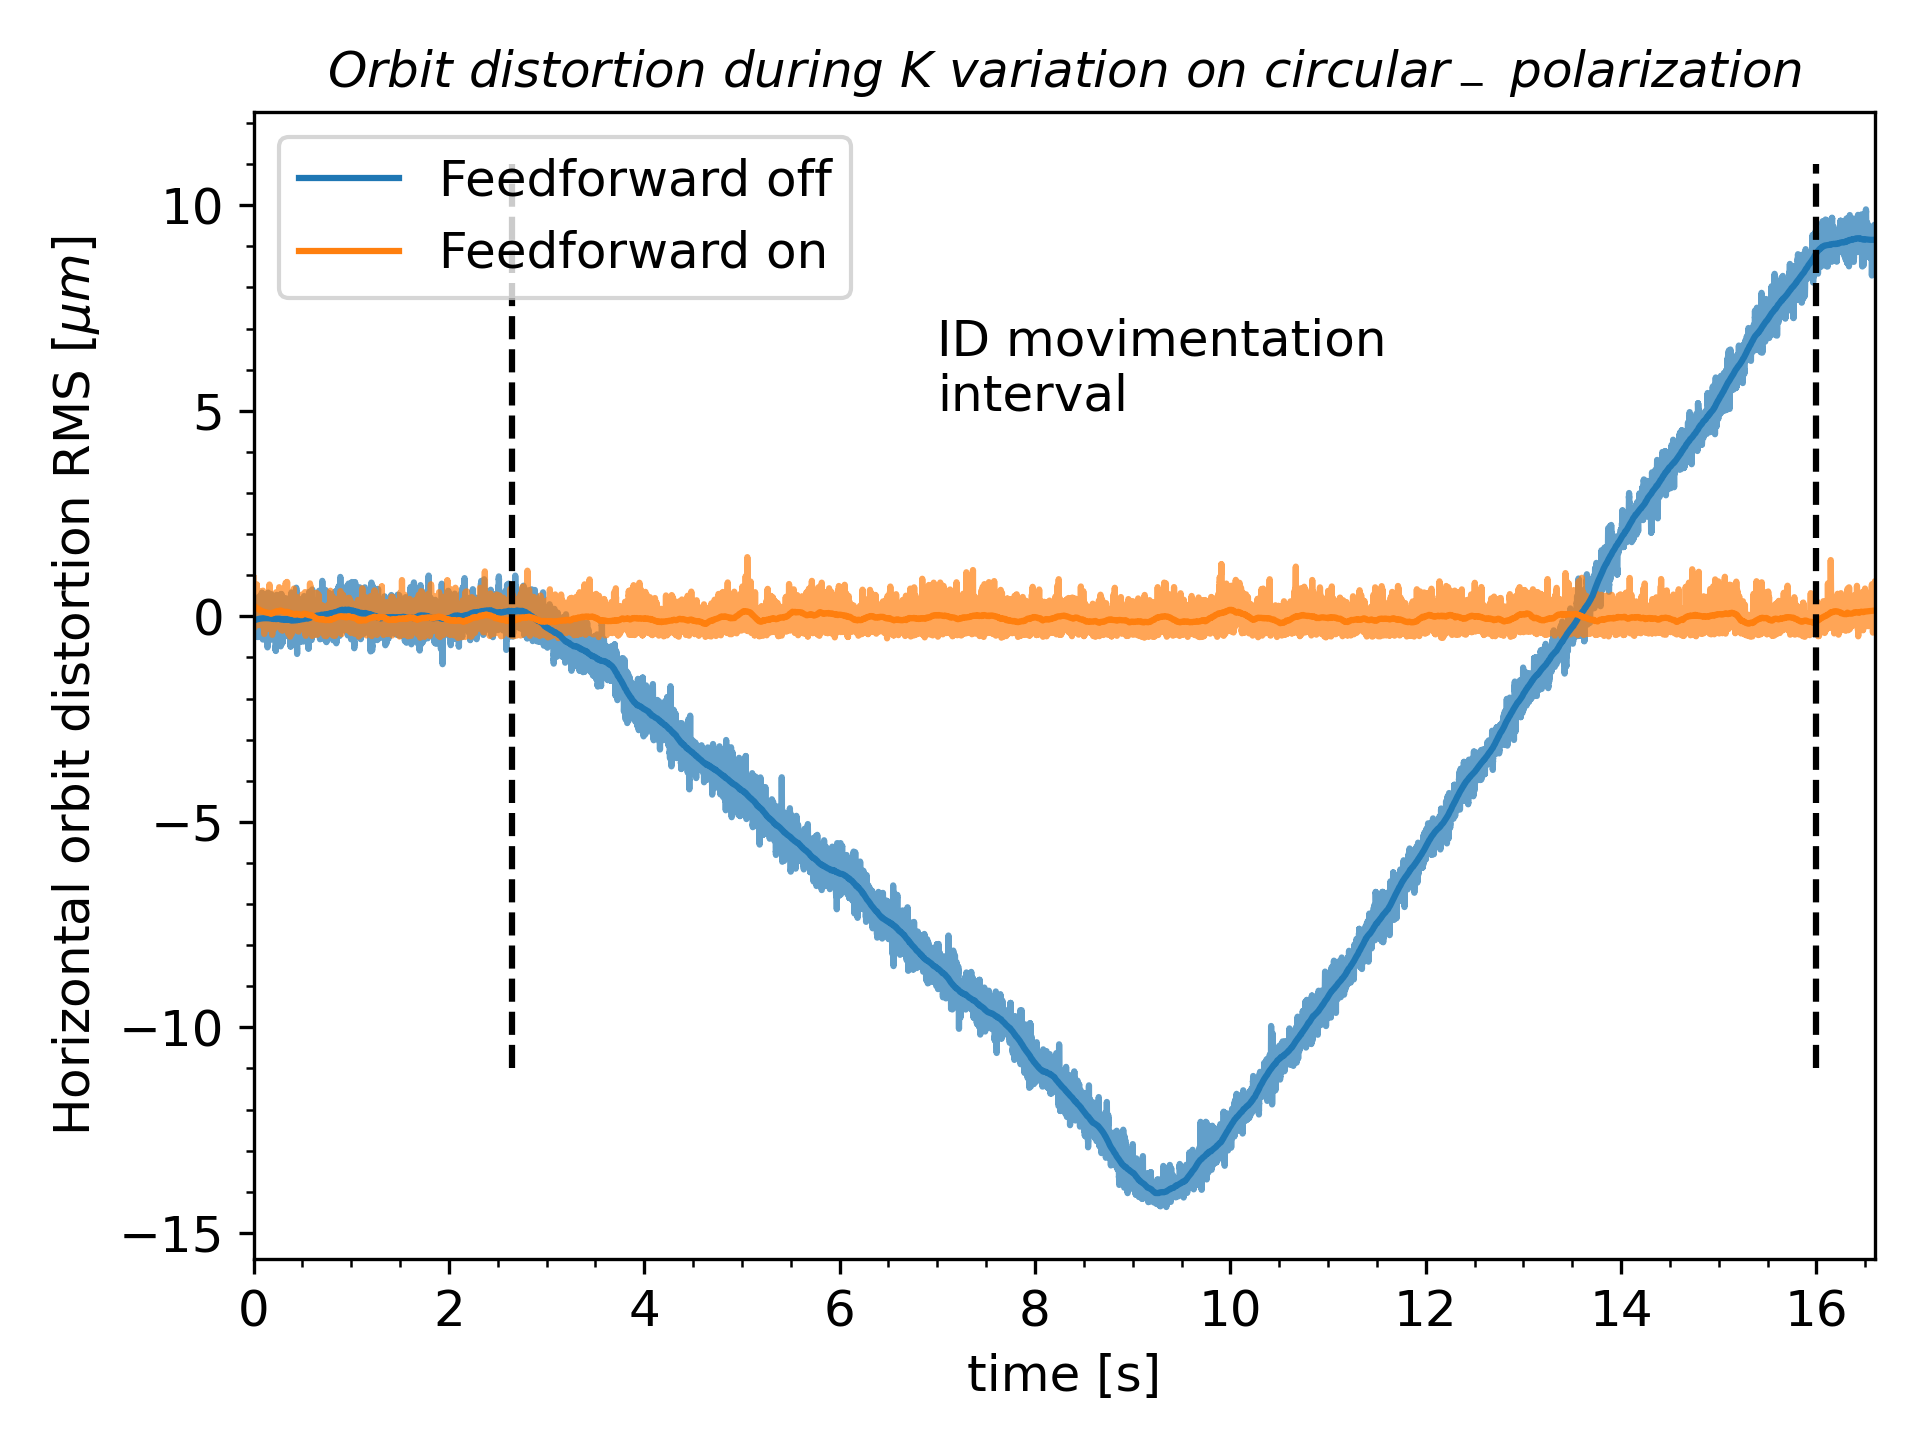
\includegraphics[width=\textwidth]{2024-05-31/figures/Orbit_dist_FAcq.png}
            \caption{Aquisições FAqc com e sem feedforward.}
            \label{fig:a}
        \end{minipage}
        \hspace{0.5cm}
        \begin{minipage}[b]{0.45\linewidth}
            \centering
            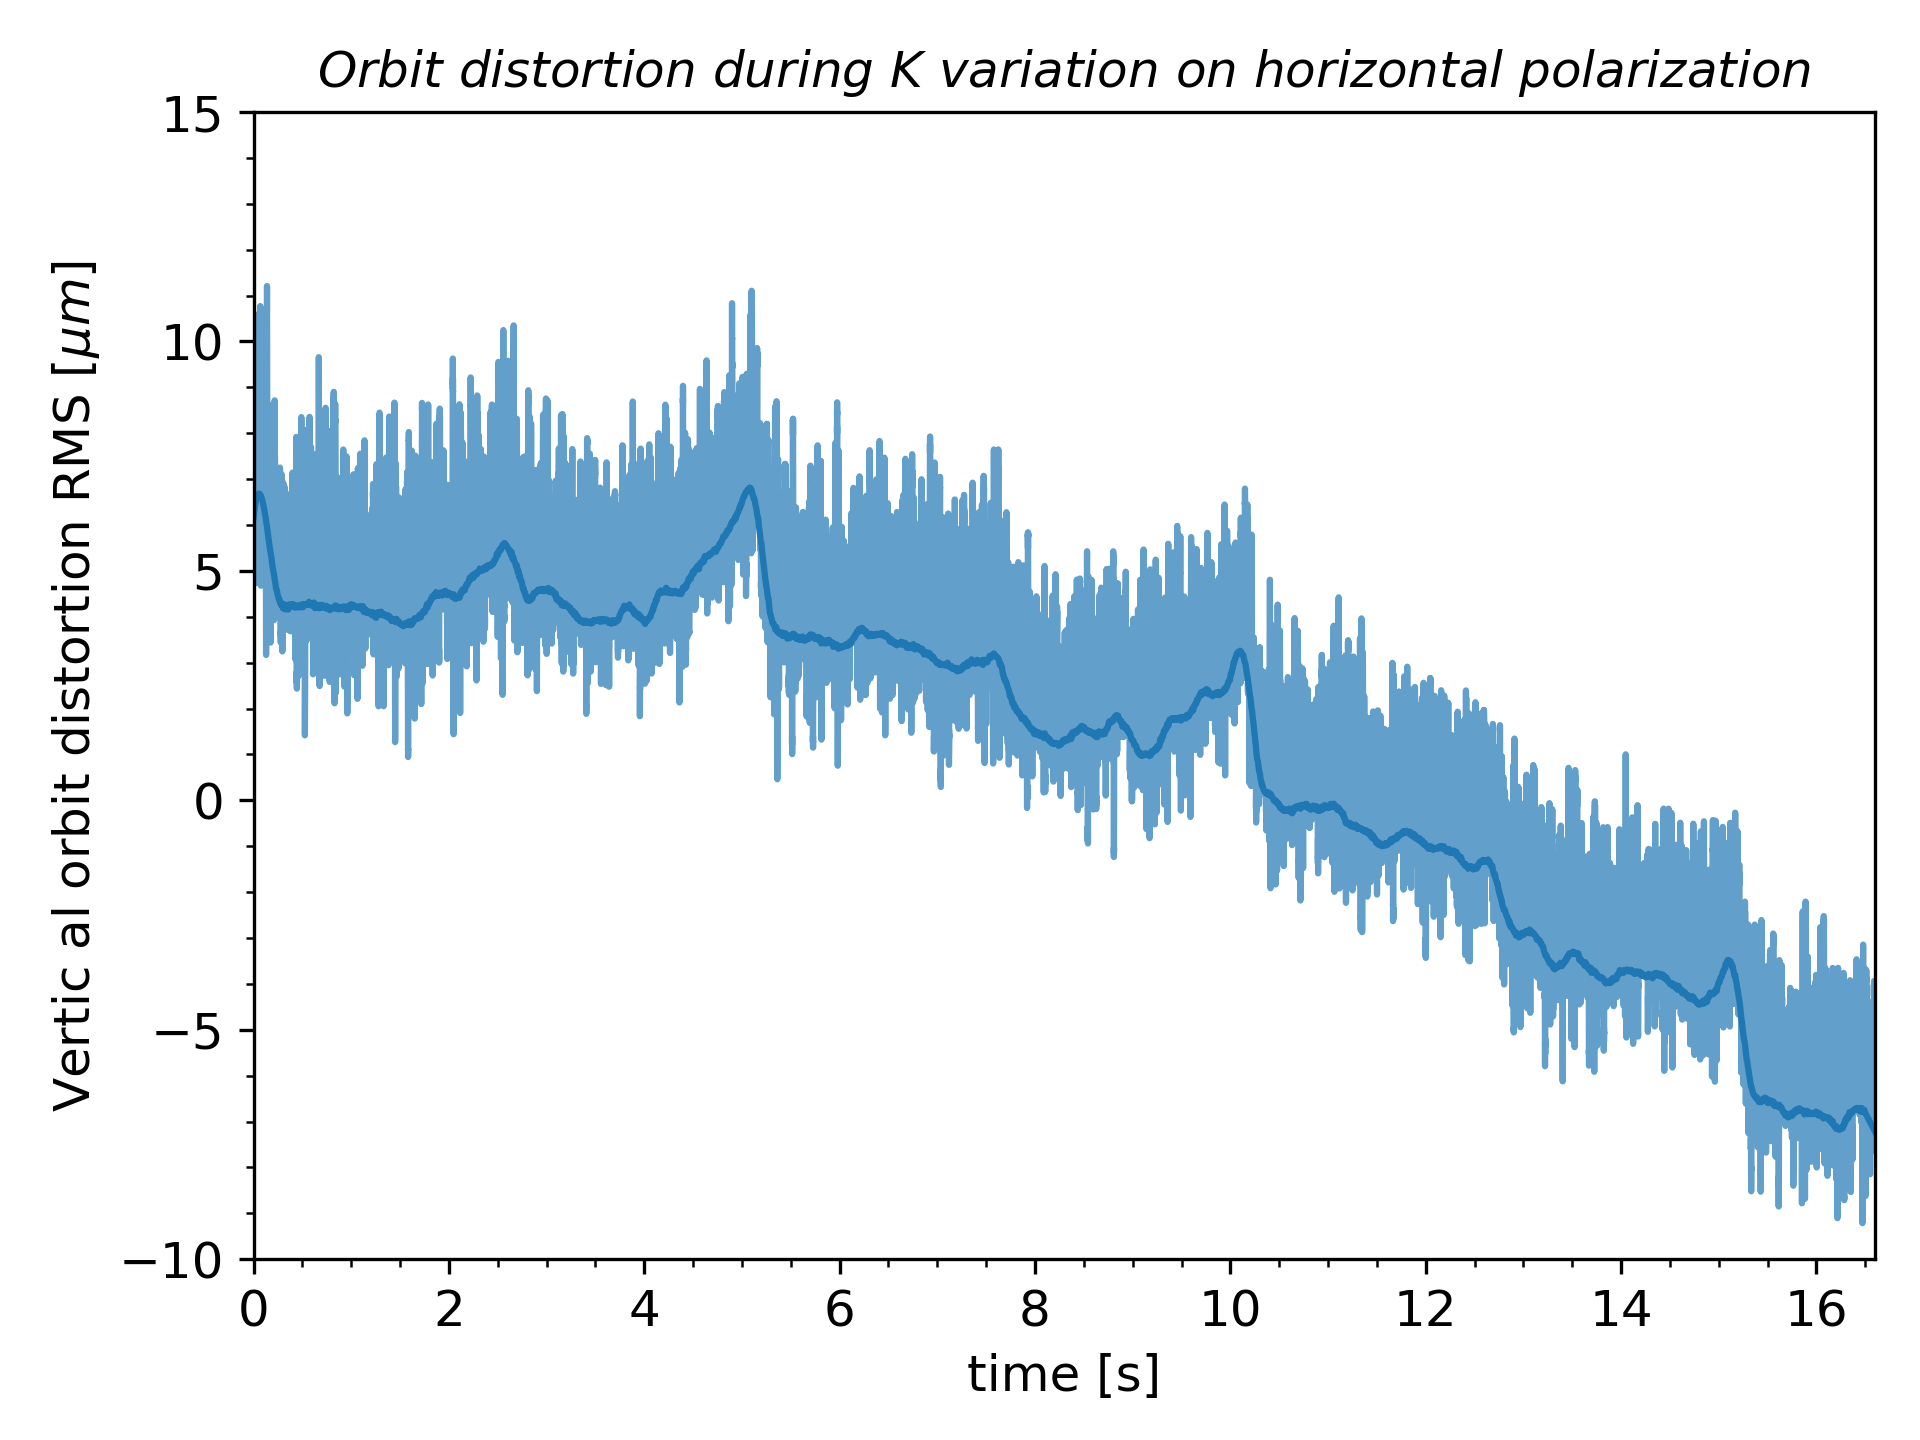
\includegraphics[width=\textwidth]{2024-05-31/figures/Orbit_dist_FAcq_bpm_disturb.png}
            \caption{Variações rápidas de órbita durante a movimentação.}
            \label{fig:b}
        \end{minipage}
    \end{figure}

\end{frame}



%====================================================================
\section{FF de sintonia para perturbação do DELTA52}

\begin{frame}{FF de tune para perturbação do DELTA52}

\begin{itemize}
    \item Estudos em 2024-04-29
\end{itemize}
\centering
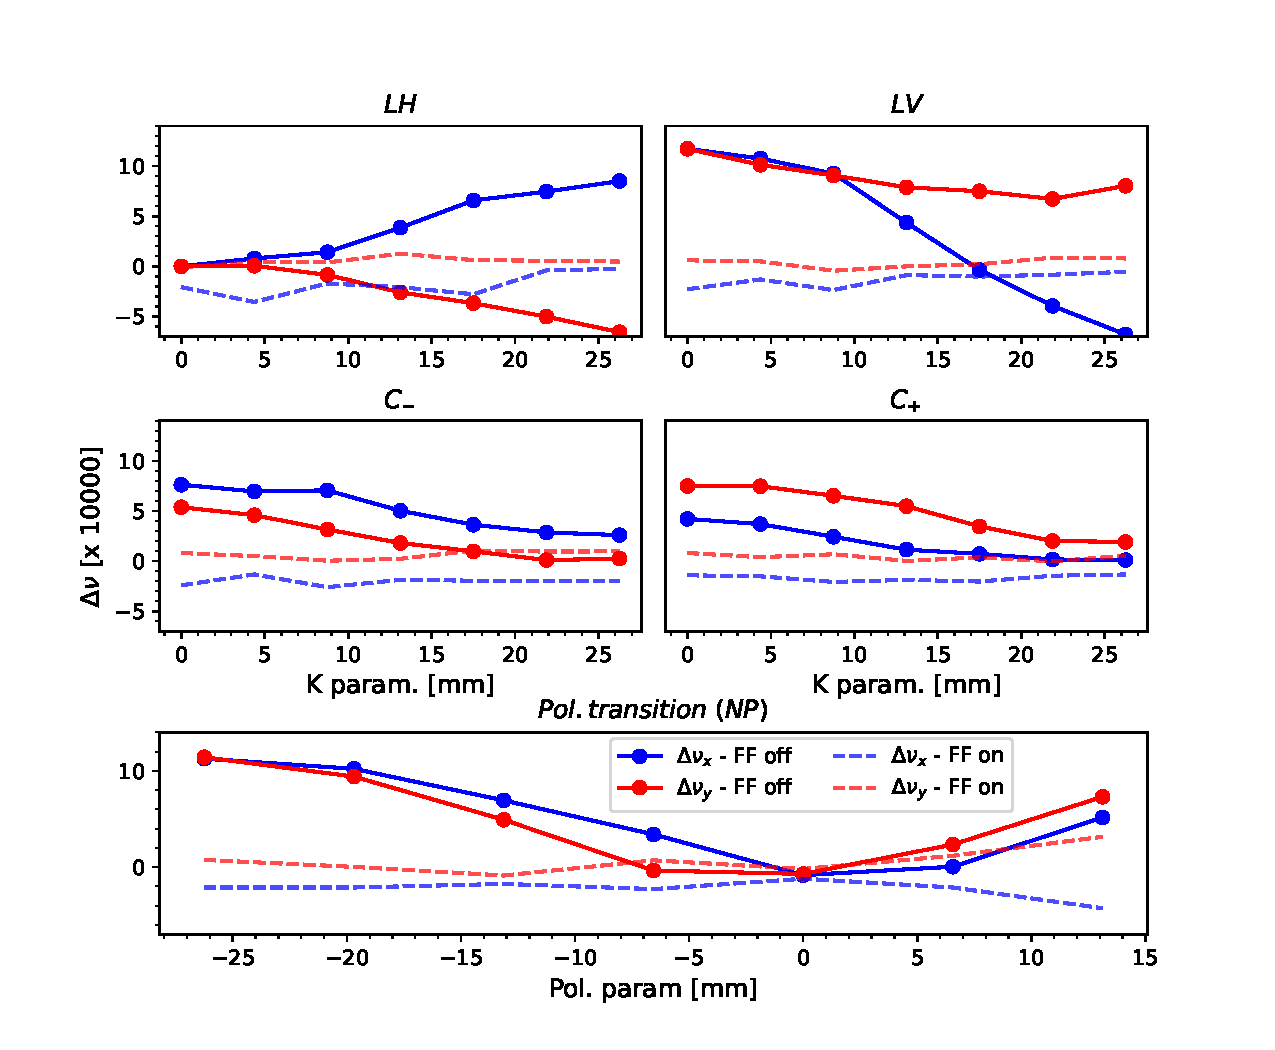
\includegraphics[scale=0.4]{2024-05-31/figures/Tune_deviation.pdf}
A variação das forças dos quadrupolos foi menor que $0.07 \%$
\end{frame}



%====================================================================
\section{Função de transferência I-B das corretoras do DELTA52}

\begin{frame}{Função de transferência I-B das corretoras do DELTA52}
\begin{itemize}
    \item Estudos em 2024-05-06
    \item Medimos a função de transferência das corretoras.
\end{itemize}
\centering
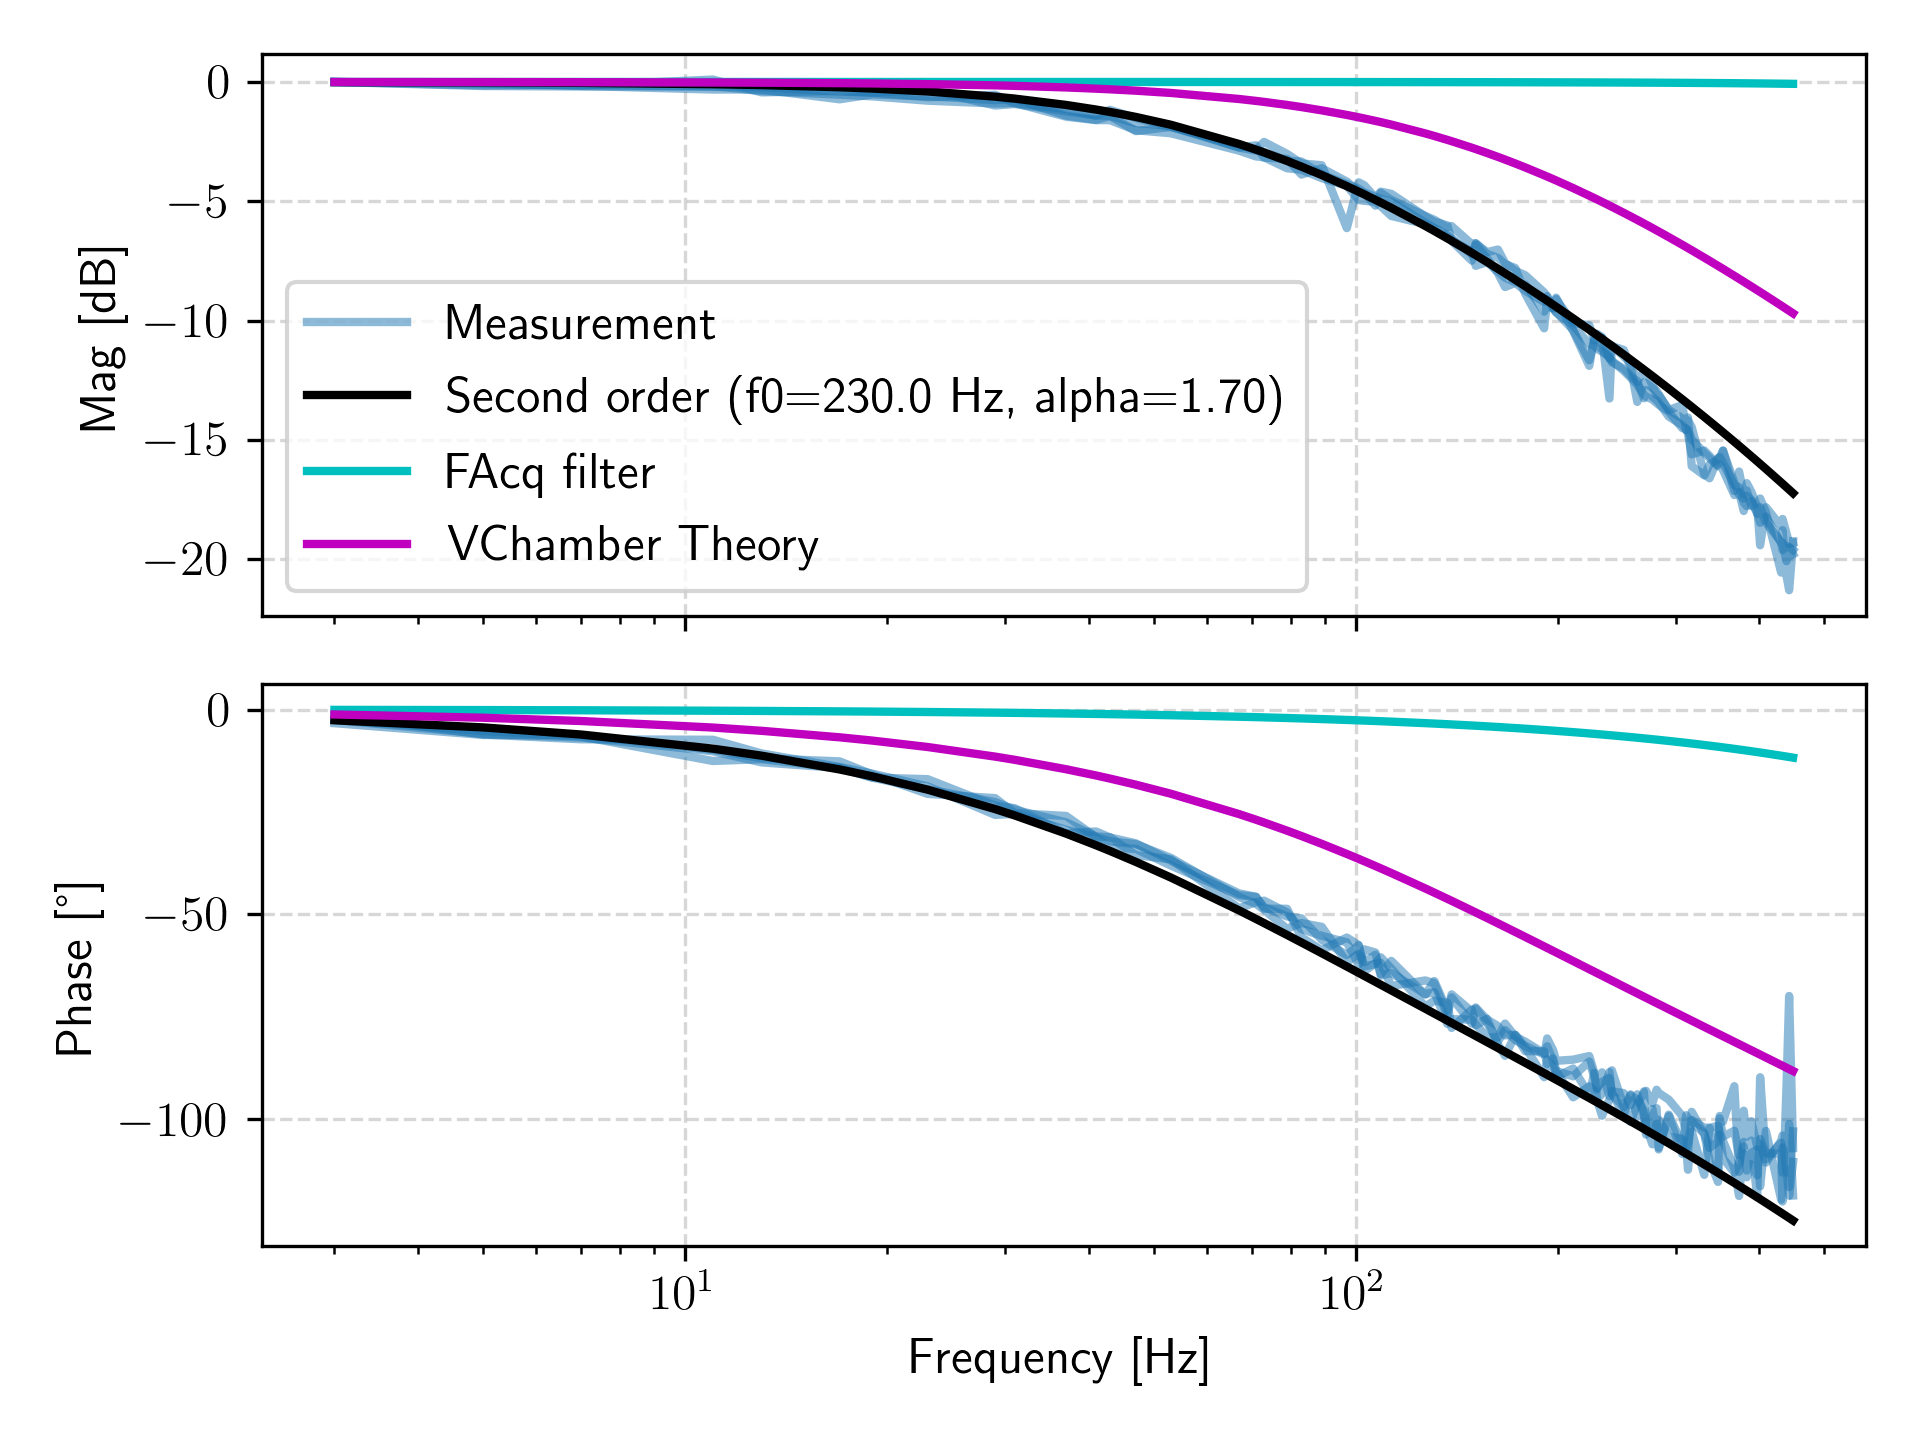
\includegraphics[scale=0.49]{2024-05-31/figures/transfer_function_delta_correctors.png}
\end{frame}



%====================================================================
\section{Compensação NLK}

\begin{frame}{Compensação NLK}

\begin{itemize}
    \setlength\itemsep{1em}
    \item Estudos em 2024-04-29, 2024-05-06; feito em paralelo a outros estudos
    \item Fizemos varreduras de atraso e amplitude mais finas e sistemáticas, medindo oscilação na taxa ADCSwap. novos valores otimizados mas sem melhoras significativas.
    \item 14/05 (terça) iremos fazer medidas na taxa TbT para reavaliar necessidade de novo realinhamento na parada de 20/05
\end{itemize}

\end{frame}



%====================================================================
\section{Aquisições TbT}

\begin{frame}{Aquisições TbT - Testes do script}
% Script para automatizar a configuração do timing dos BPMs e pingers, forças dos pingers e 
% realizar aquisição triggerada de dados volta-a-volta para analisar ótica linear, i.e., 
% beta-beating e erros de fase nos BPMs (implementado), e energy-spread, tune-shifts e (talvez) 
% emitâncias (ainda não implementados) 
% \pause
    \begin{itemize}
        \setlength\itemsep{1em}
        \item 2024-22-04: primeiros testes, dificuldades na automatização da medida devido à rampa lenta dos pulsados e checagem do readback das forças.
        % \pause
        \item 2024-29-04: checagem do Mon das forças, aquisições bem sucedidas, falha em restaurar estado pré-medida (bug de código). 
        \begin{itemize}
            \item análise dos dados adquiridos indicavam algumas anomalias (próximo slide)
        \end{itemize}
        % \pause
        \item 2024-06-05: script debugado, medida e restauração do estado inicial funcionando. 
         \begin{itemize}
            \item amplitudes ainda são menores do que o valor esperado (comparação com aquisições passadas)
            \item aquisições e kicks no continuous não apresentam esse problema.
        \end{itemize}
    \end{itemize}
\end{frame}

\begin{frame}{Aquisições TbT - ``Anomalia`` (29/04)}
{\tiny Comparação PCA vs ICA, medida com anomalia (provavelmente de aquisição) (do erro de fase em escala separada) } 
    \begin{figure}
        \centering
        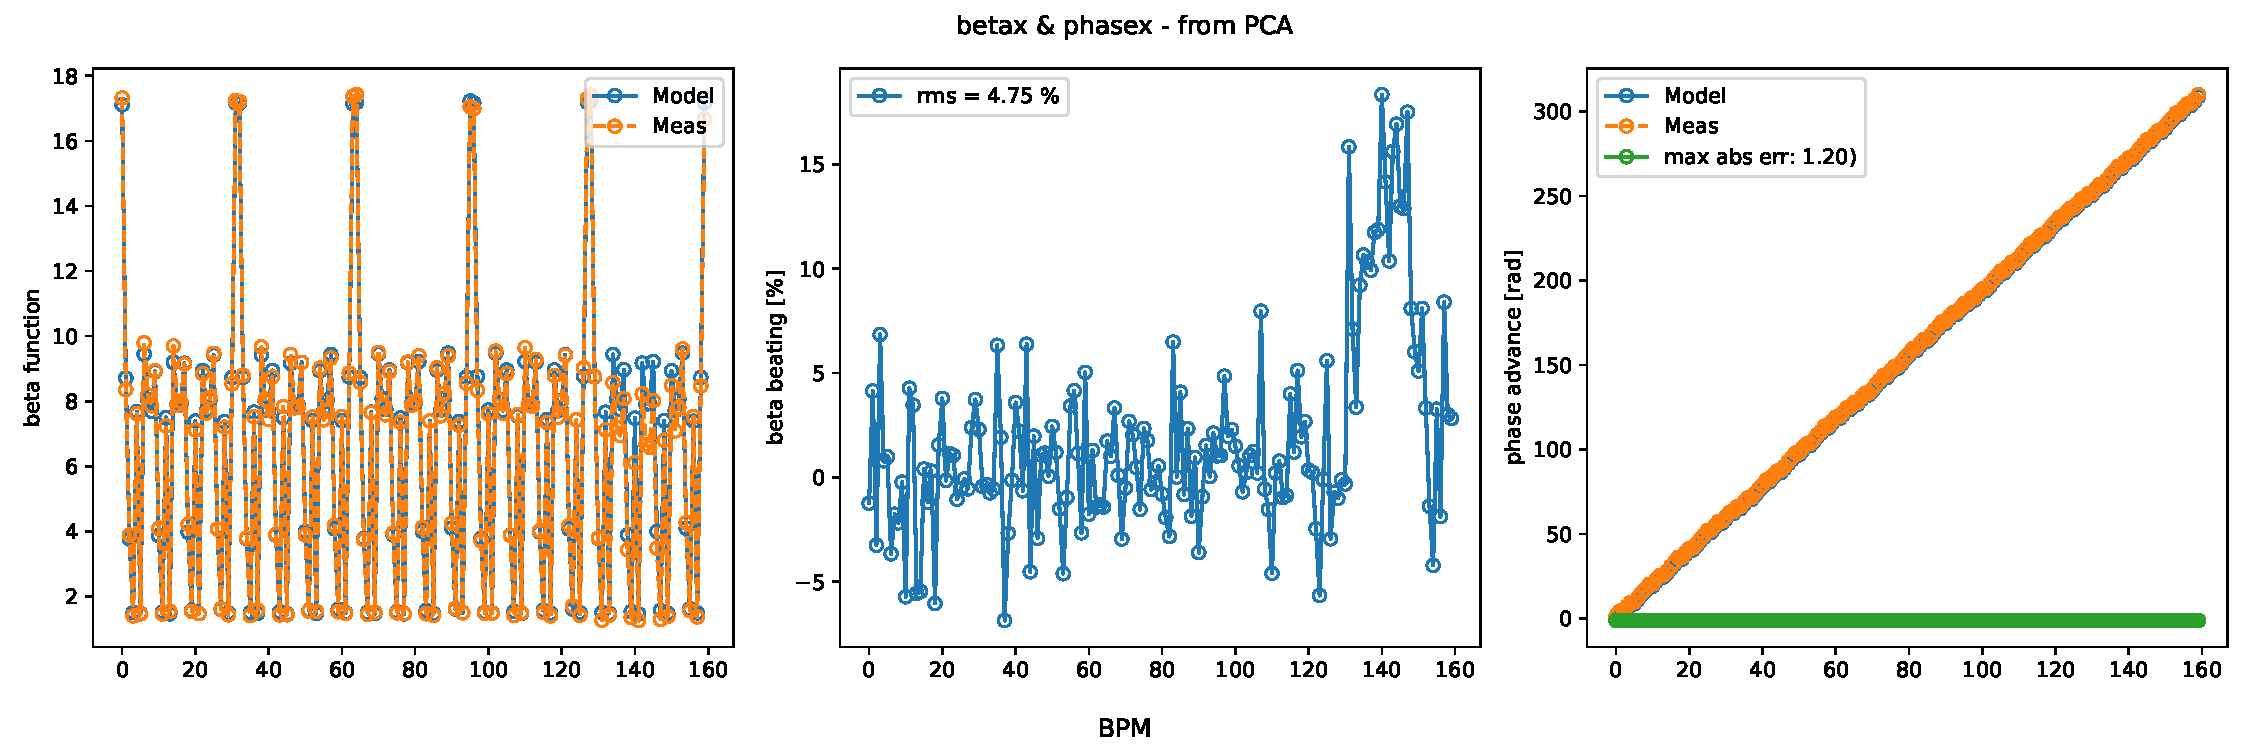
\includegraphics[width=0.75\textwidth]{2024-05-31/figures/beta_beat_PCA_050urad_kickh_290424.pdf}
    \end{figure}
    \begin{figure}
        \centering
        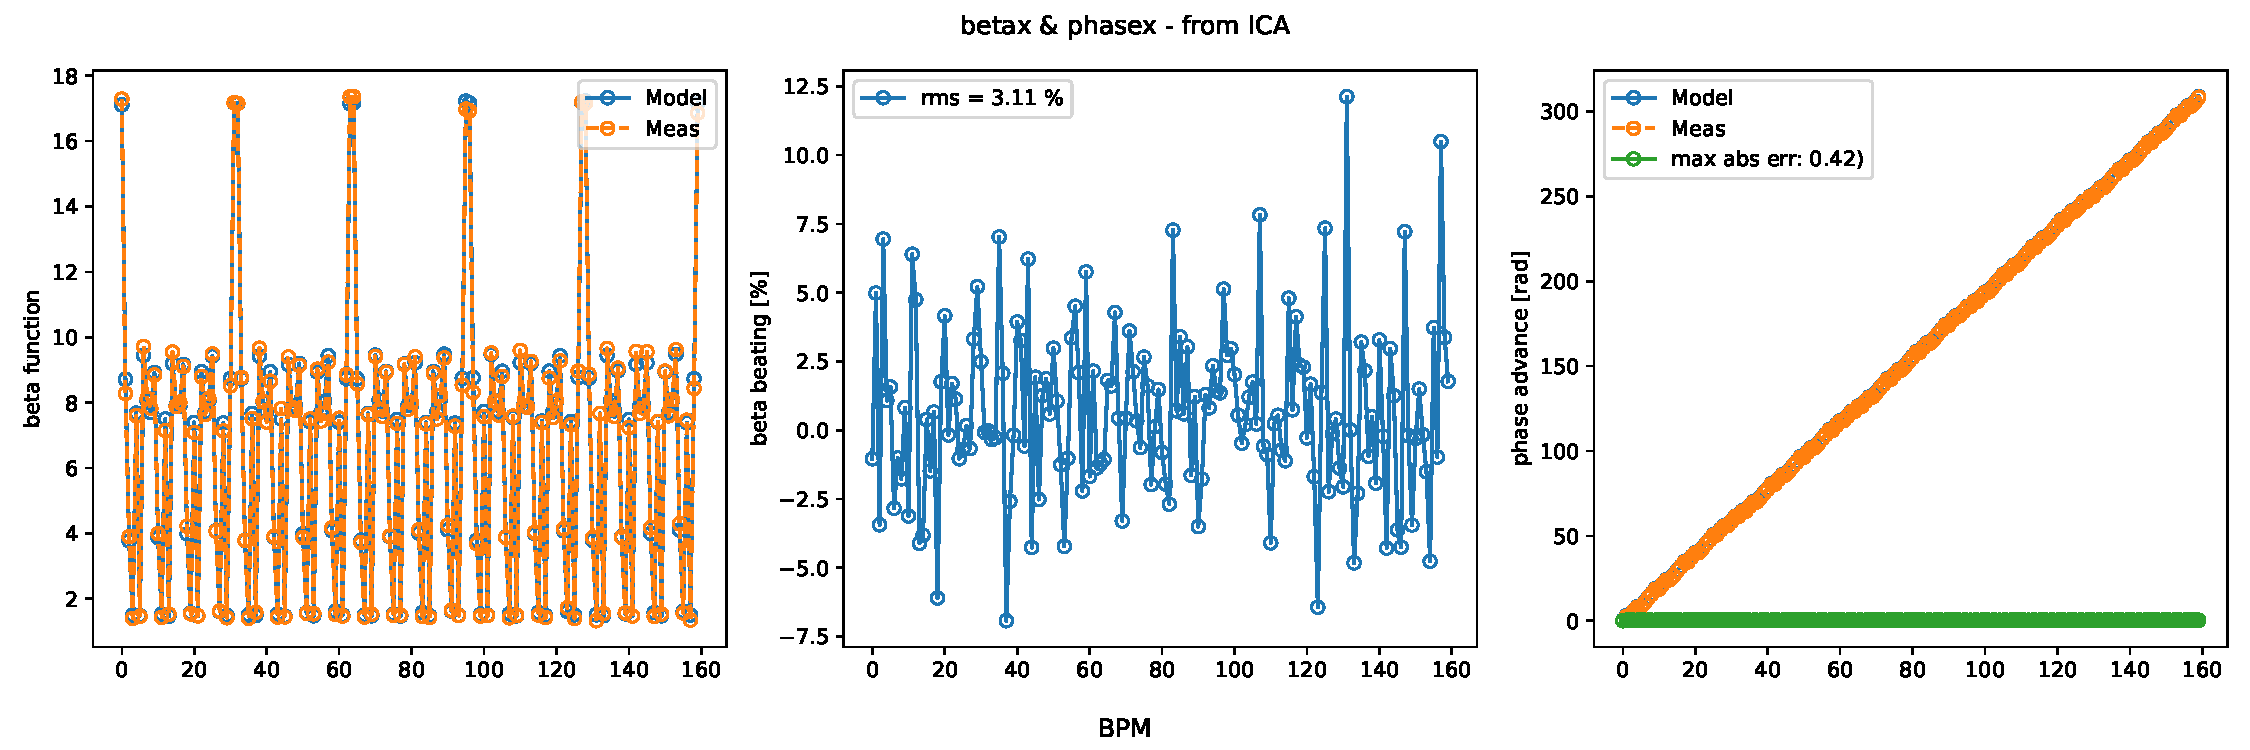
\includegraphics[width=0.75\textwidth]{2024-05-31/figures/beta_beat_ICA_050urad_kickh_290424.pdf}
    \end{figure}
\end{frame}

\begin{frame}{Aquisições TbT - (06/05)}
{\tiny Comparação PCA de medida normal (06/05) vs ICA de medida anômala (29/04)}
\begin{figure}
        \centering
        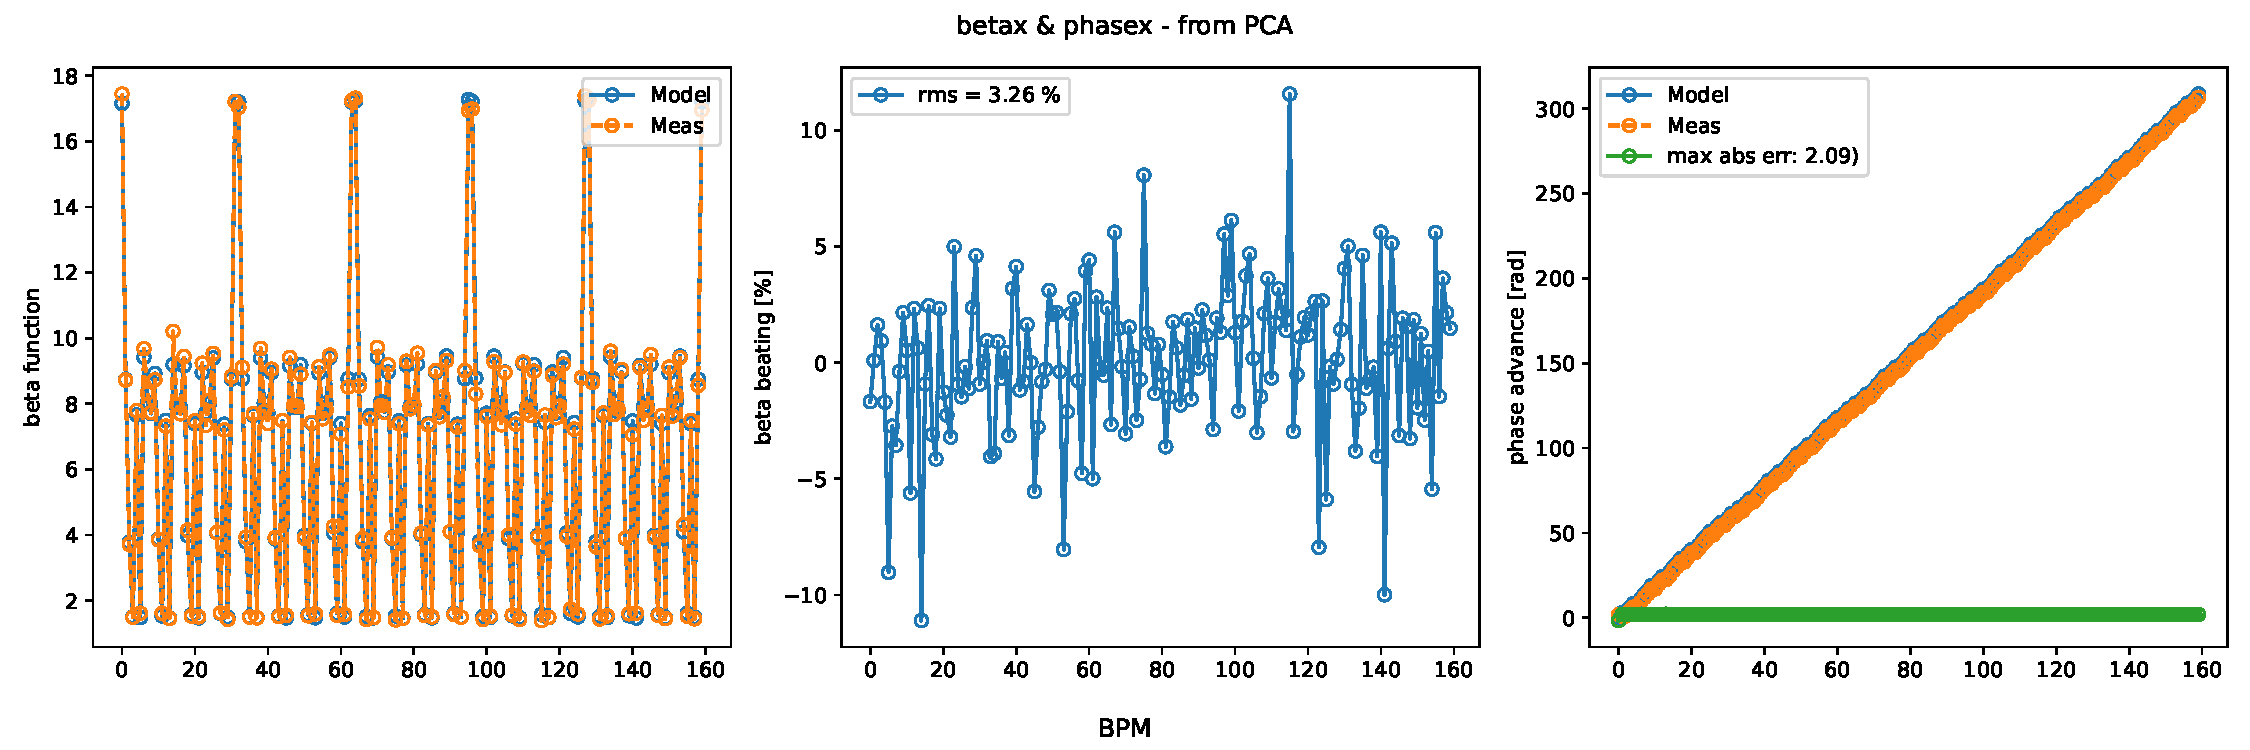
\includegraphics[width=0.75\textwidth]{2024-05-31/figures/beta_beat_PCA_100urad_kickh_060524.pdf}
    \end{figure}
    \begin{figure}
        \centering
        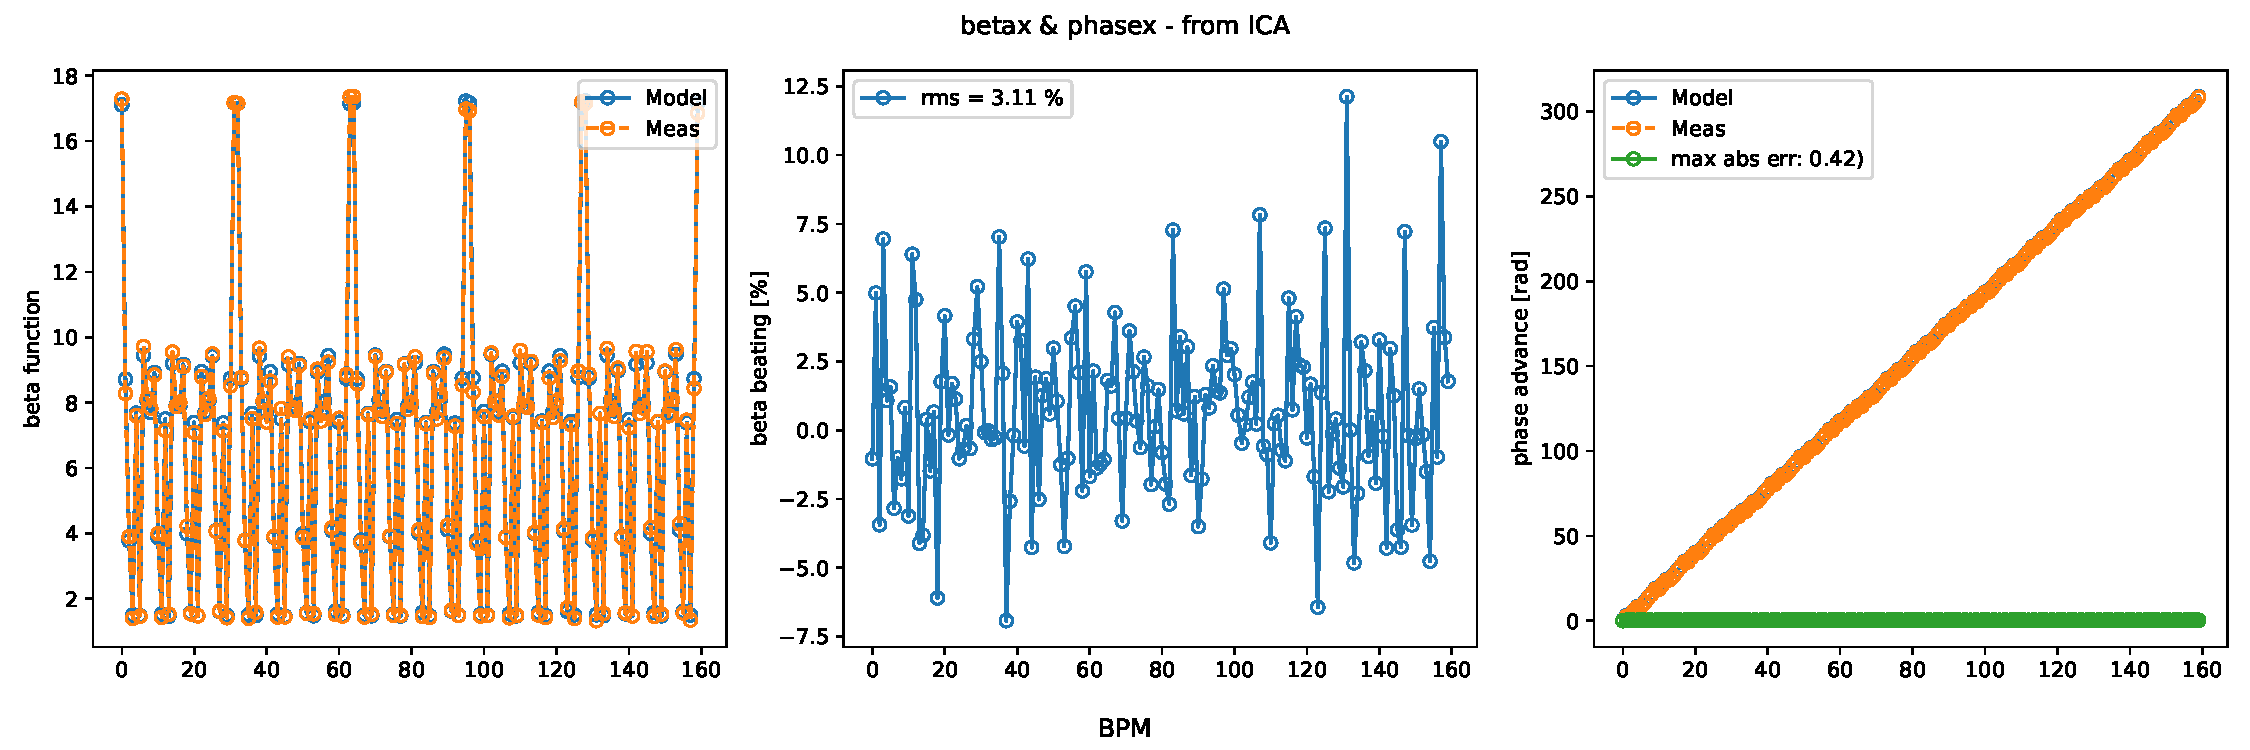
\includegraphics[width=0.75\textwidth]{2024-05-31/figures/beta_beat_ICA_050urad_kickh_290424.pdf}
    \end{figure}
\end{frame}

\begin{frame}{Aquisições TbT - TODO's}
Análises
    \begin{itemize}
        \setlength\itemsep{1em}
        \item Barras de erro para $\Delta \beta/\beta$ e $\Delta \phi$
        % \item ICA depende da identificação visual de modos senoidais e cossenoidais: ainda não-automatizado;
        \item Estudo de sensitividade e robustez: ICA vs PCA 
        \begin{itemize}
            \item Sensitividade de $\Delta \beta / \beta$ e $\Delta \phi$ por $\Delta KL$
            \item Robustez a ruido e fontes contaminantes no sinal TbT
            \item Comparação com sensitividade e robustez do LOCO
        \end{itemize}
        \item Estudos com modelo sobre a viabilidade de usar essas ferramentas para um esquema de correção
    \end{itemize}
\vfill
Medida
    \begin{itemize}
        \setlength\itemsep{1em}
        \item Entender o porquê das amplitudes menores do que esperadas 
    \end{itemize}
\end{frame}



%====================================================================
\section{Estudo da correção da órbita do booster}

\begin{frame}{Correção com deslocamento dos quadrupolos}
    \begin{itemize}
        \item Problemas com uso da classe de cálculo de matriz resposta;
        \item Determinação da sequência de quadrupolos que melhor corrigem a órbita.
    \end{itemize}
    \begin{minipage}{\textwidth}
        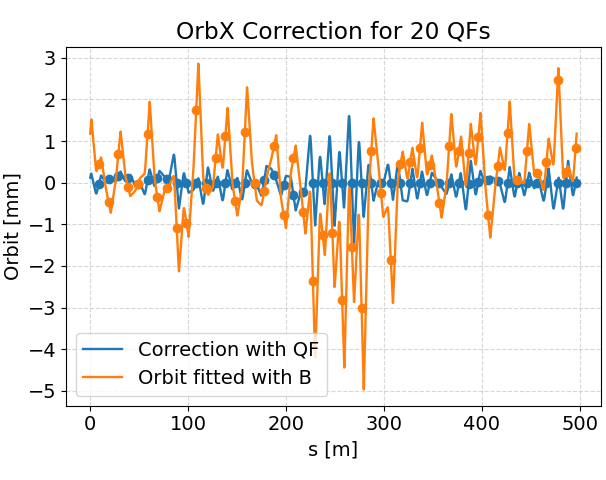
\includegraphics[width=0.5\linewidth]{2024-05-31/figures/qf_orbit_correction.png}
        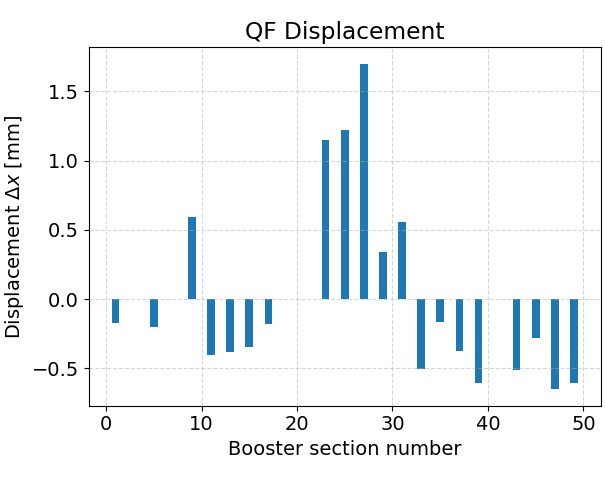
\includegraphics[width=0.5\linewidth]{2024-05-31/figures/qf_displacement.png}
    \end{minipage}
    Próximos passos
    \begin{itemize}
        \item Analisar o efeito de erros de offset de BPMs na órbita residual;
        \item Análisar as medidas de campo dos dipolos instalados no booster.
    \end{itemize}
\end{frame}



\end{document}